\appendix
\section{Apéndices}

\subsection{Modelo Canvas}

La Figura~\ref{fig:canvas} sintetiza los nueve bloques desarrollados en el cuerpo
del informe. Sus precios, capacidades y límites corresponden al modelo vigente;
las condiciones comerciales definitivas dependen de la validación del piloto.

\begingroup
\centering
\vspace*{0.5cm}
\begingroup
\newcommand{\bloquecanvas}[2]{%
\begin{minipage}[t]{0.32\textwidth}
\begin{tcolorbox}[colback=white,colframe=teal!65!black,colbacktitle=teal!65!black,
coltitle=white,title={#1},fonttitle=\bfseries\small,height=3.9cm,
left=1.3mm,right=1.3mm,top=1.3mm,bottom=1.3mm]
\small\setstretch{1}\raggedright #2
\end{tcolorbox}
\end{minipage}}
\bloquecanvas{Segmentos}{Dueños y administradores.\\[2mm]
Entrenadores y miembros.\\[2mm]
Validación inicial: Pérez Zeledón.}
\hfill
\bloquecanvas{Propuesta de valor}{Membresías, pagos, asistencia, rutinas y progreso.\\[2mm]
Acceso web por rol.\\[2mm]
Acompañamiento inicial.}
\hfill
\bloquecanvas{Canales}{Contacto directo y demostración.\\[2mm]
Página, redes y mensajería.\\[2mm]
Entrega web y soporte digital.}

\smallskip
\bloquecanvas{Relaciones}{Configuración guiada.\\[2mm]
Piloto de cuatro semanas propuesto.\\[2mm]
Seguimiento e incidencias.\\[2mm]
Prueba pendiente.}
\hfill
\bloquecanvas{Ingresos}{Mensualidades proyectadas:\\[2mm]
Starter: CRC 15\,000.\\
Pro Gym: CRC 25\,000.\\[2mm]
Mezcla: un Starter y los demás Pro Gym.}
\hfill
\bloquecanvas{Recursos}{Equipo y tutoría académica.\\[2mm]
Código, equipos y nube.\\[2mm]
Separación de datos por gimnasio pendiente.}

\smallskip
\bloquecanvas{Actividades}{Investigar y desarrollar.\\[2mm]
Probar y documentar.\\[2mm]
Demostrar y dar soporte.\\[2mm]
Revisar costos y calidad.}
\hfill
\bloquecanvas{Alianzas}{Tutor: colaboración confirmada.\\[2mm]
Gimnasio aliado: pendiente.\\[2mm]
Nube: proveedores de servicio.}
\hfill
\bloquecanvas{Costos}{Base mensual: CRC 114\,247,54.\\[2mm]
Costos según clientes.\\[2mm]
Desarrollo: CRC 198\,735,27.\\
Trabajo aportado sin pago.}
\par
\endgroup

\captionof{figure}{Modelo Canvas vigente de Pulso}
\label{fig:canvas}
\caption*{\textit{Nota}. Elaboración propia a partir del escenario financiero preliminar.}
\par
\endgroup
\clearpage

\subsection{Ruta comercial propuesta}

\begin{figure}[htbp]
\centering
\newcommand{\pasorutacomercial}[4]{%
  \begin{tcolorbox}[enhanced,arc=1.2mm,boxrule=0.7pt,
    colback=#3,colframe=#4,colbacktitle=#4,coltitle=white,
    fonttitle=\bfseries\small,title={#1},
    width=\linewidth,height=1.9cm,top=1.4mm,bottom=1.2mm,left=1.5mm,right=1.5mm]
    \centering\sffamily\small #2
  \end{tcolorbox}%
}
\begin{minipage}[c]{0.205\textwidth}
\pasorutacomercial{Contacto}{Visita o mensaje}{teal!6}{teal!65!black}
\end{minipage}\hfill
{\color{teal!65!black}\Large$\longrightarrow$}\hfill
\begin{minipage}[c]{0.205\textwidth}
\pasorutacomercial{Demostración}{Datos ficticios}{cyan!8}{cyan!60!black}
\end{minipage}\hfill
{\color{teal!65!black}\Large$\longrightarrow$}\hfill
\begin{minipage}[c]{0.205\textwidth}
\pasorutacomercial{Piloto}{4 semanas}{orange!10}{orange!75!black}
\end{minipage}\hfill
{\color{teal!65!black}\Large$\longrightarrow$}\hfill
\begin{minipage}[c]{0.205\textwidth}
\pasorutacomercial{Suscripción}{Soporte y revisión}{green!8}{green!50!black}
\end{minipage}
\caption{Ruta comercial propuesta de Pulso}
\label{fig:ruta-comercial}
\caption*{\textit{Nota}. Elaboración propia. Resume los pasos previstos para ofrecer el servicio.}
\end{figure}

\subsection{Instrumento de validación}

Las encuestas se aplicaron a dueños o administradores de gimnasios,
entrenadores personales y clientes o miembros de gimnasios. Se obtuvieron
15 respuestas válidas: cinco de responsables y diez de miembros.

\begin{longtable}{>{\bfseries}p{1.5cm}p{8cm}p{4.5cm}}
\caption{Transcripción normalizada del instrumento aplicado}\label{tab:instrumento-resumen}\\
\toprule
Código & Pregunta & Tipo u opciones \\
\midrule
\endfirsthead
\toprule
Código & Pregunta & Tipo u opciones \\
\midrule
\endhead
C1 & ¿Tiene 18 años o más y acepta participar voluntariamente? & Opción única: sí o no; una negativa finaliza la participación. \\
C2 & ¿Desde cuál rol responde? & Dueño o administrador; entrenador con responsabilidades administrativas; entrenador independiente; miembro. \\
C3 & ¿Dónde se ubica principalmente el gimnasio con el que se relaciona? & Pérez Zeledón; otro cantón de San José; otra provincia. \\
A1 & ¿Cuántos miembros activos administra aproximadamente? & 1--25; 26--75; 76--150; más de 150; no sabe o no aplica. \\
A2 & ¿Qué herramientas utiliza actualmente para administrar el gimnasio o sus clientes? & Selección múltiple: papel, hoja de cálculo, WhatsApp, software, sistema interno u otra. \\
A3 & ¿Cuáles tareas le generan mayor dificultad o tiempo? & Selección múltiple de tareas administrativas y deportivas. \\
A4 & ¿Con qué frecuencia ocurren errores, atrasos o confusiones por la gestión actual? & Escala de 1, nunca, a 5, muy frecuentemente. \\
A5 & ¿Qué funciones serían más valiosas en una plataforma? & Selección múltiple; se analizaron únicamente las categorías que la exportación permitió distinguir. \\
A6 & ¿Desde qué dispositivo esperaría administrar principalmente el sistema? & Celular, computadora, tableta o combinación. \\
A7 & ¿Estaría dispuesto a probar durante cuatro semanas una plataforma con datos de demostración y acompañamiento? & Sí, según condiciones, tal vez o no. \\
A8 & Si la plataforma resolviera las funciones seleccionadas, ¿qué rango mensual consideraría razonable? & Rangos desde menos de CRC 7\,500 hasta CRC 40\,000 o más; no pagaría; requiere demostración. \\
A9 & ¿Qué apoyo sería más importante para adoptar la plataforma? & Selección múltiple de configuración, capacitación, soporte, tutoriales, respaldo y personalización. \\
A10 & ¿Qué tan importante considera controlar quién accede a datos de miembros, pagos y progreso? & Muy importante, importante, poco importante o no sabe. \\
A11 & ¿Qué condición tendría que cumplir Pulso para ser útil en su trabajo? & Respuesta abierta opcional. \\
B1 & ¿Con qué frecuencia asiste normalmente al gimnasio? & Menos de una vez; 1--2; 3--4; o 5 o más veces por semana. \\
B2 & ¿Qué información puede consultar actualmente de forma digital? & Selección múltiple sobre membresía, pagos, asistencia, rutina, progreso, mensajes, ninguna u otra. \\
B3 & ¿Qué situaciones le generan mayor dificultad? & Selección múltiple sobre vencimientos, pagos, rutina, sesiones, progreso, comunicación u otra. \\
B4 & ¿Desde qué dispositivo utilizaría Pulso? & Celular, computadora, tableta o no la usaría. \\
B5 & ¿Qué tan útil sería reunir pagos, asistencia, rutina y progreso en un solo lugar? & Escala de 1, nada útil, a 5, muy útil. \\
B6 & ¿Qué función haría que utilizara una aplicación de un gimnasio? & En la versión aplicada quedó configurada como respuesta abierta y no como categorías comparables. \\
B7 & ¿Qué haría que utilizara o dejara de utilizar una aplicación de gimnasio? & Respuesta abierta opcional. \\
\bottomrule
\caption*{\textit{Nota}. Se corrigieron tildes y errores mecanográficos para facilitar la lectura, sin modificar los datos. La versión aplicada no incluyó la pregunta de privacidad para miembros. La exportación original permanece en \texttt{resultado\_encuesta.csv}.}
\end{longtable}

\subsection{Limitaciones metodológicas de la encuesta}

La selección se hizo por acceso a las personas y participación voluntaria,
sin sorteo; por eso la muestra es no probabilística y por conveniencia.
Respondieron más miembros que responsables. Varios dueños rechazaron
participar y no se anotó el total de invitaciones ni de rechazos, por lo que
no se pudo calcular una tasa de respuesta. Los resultados describen a las
15 personas consultadas y no se pueden extender a todos los gimnasios de
Pérez Zeledón.

La versión aplicada en Google Forms presentó dos diferencias frente al
instrumento previsto: la ruta de miembros no incluyó la pregunta de privacidad y
una pregunta sobre funciones combinó opciones y respuestas abiertas de forma
inconsistente. Por eso se compararon solo las respuestas que podían agruparse
con claridad. La exportación original se conserva sin cambios y los gráficos
se generan desde esos datos.

\Needspace{12\baselineskip}
\subsection{Evidencia técnica disponible}

\begin{table}[htbp]
\caption{Inventario de evidencia técnica}
\begin{tabularx}{\textwidth}{>{\bfseries}p{4cm}X p{3cm}}
\toprule
Evidencia & Descripción & Estado \\
\midrule
Repositorio & Código frontend, backend, infraestructura y documentación. & Disponible \\
Pruebas backend & Suite automatizada de reglas de negocio, permisos y recorridos de miembros, planes, facturación y asistencia. & Se ejecuta antes de la captura \\
Pruebas frontend & Suite automatizada de componentes, pantallas y permisos por contexto. & Se ejecuta antes de la captura \\
Pruebas E2E & Recorridos de instructor y cliente en Playwright. & Se ejecuta antes de la captura \\
Frontend público & Despliegue demostrativo en Vercel. & Disponible \\
Backend y API & Despliegue y documentación OpenAPI. & Disponible \\
Capturas anonimizadas & Panel administrativo, gestión de planes del instructor y panel del cliente, con datos ficticios. & Disponible \\
\bottomrule
\end{tabularx}
\caption*{\textit{Nota}. Elaboración propia a partir del repositorio y de la versión local de demostración al 23 de septiembre de 2026 \parencite{gymhub_repo}.}
\end{table}

\Needspace{16\baselineskip}
\subsection{Capturas de la interfaz de demostración}

Las capturas complementan la descripción técnica del informe y muestran la
versión local comprobada para la etapa regional, con cuentas y datos ficticios.

\begin{figure}[htbp]
\centering
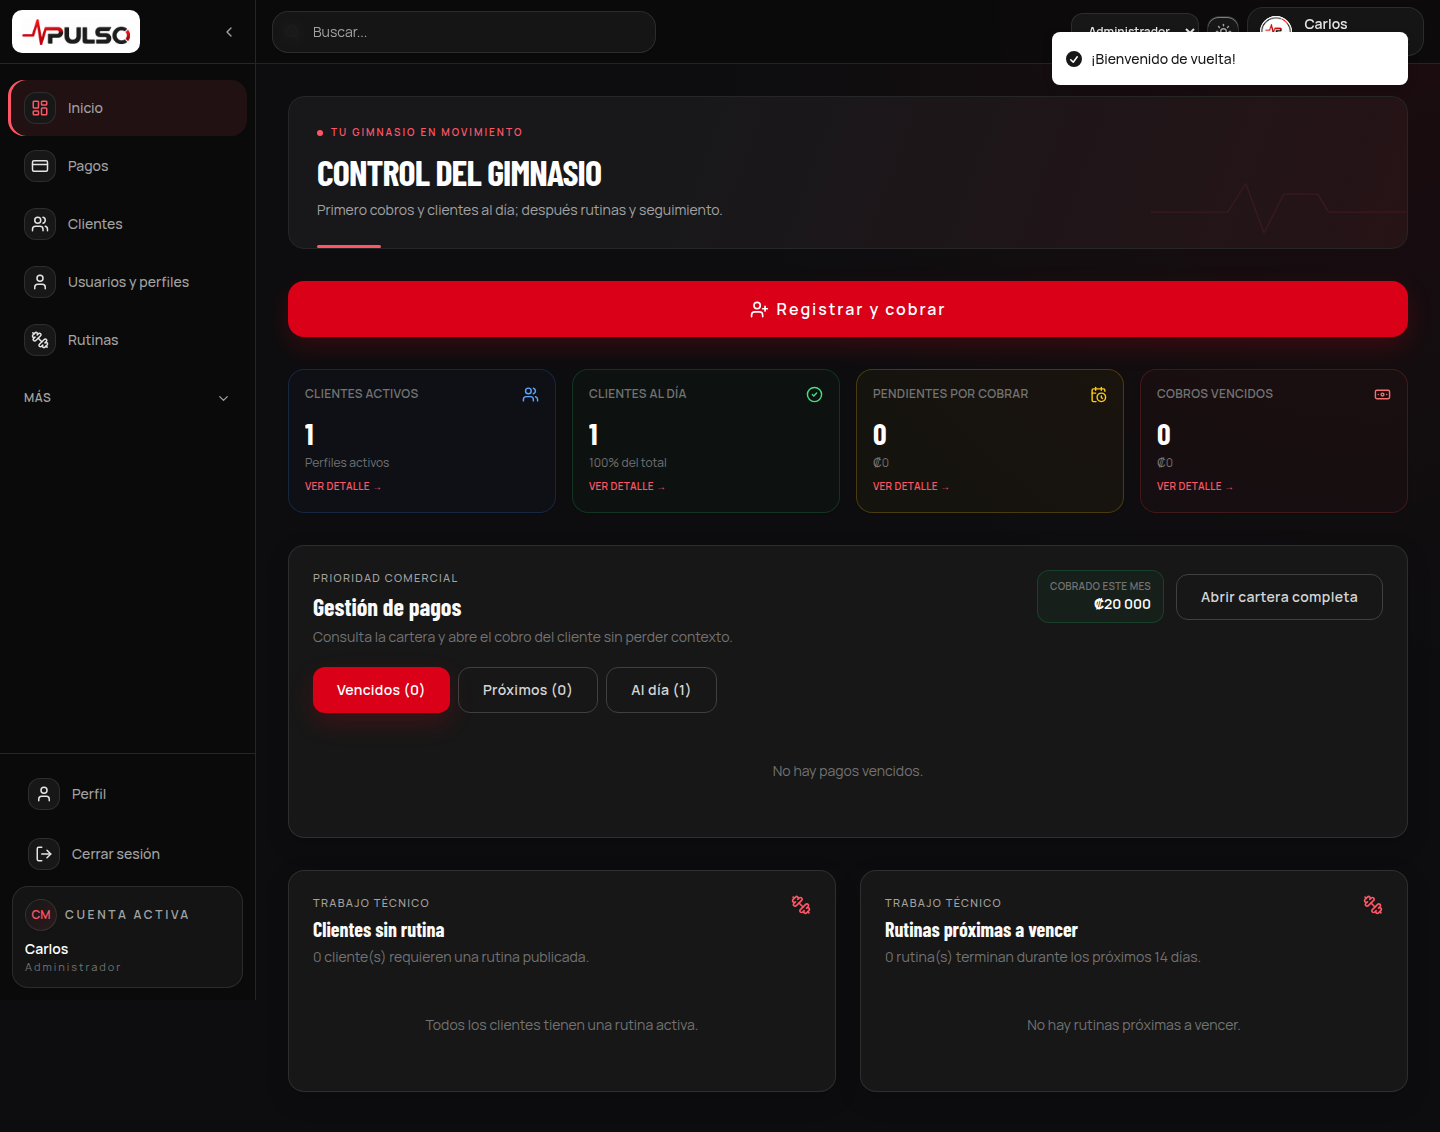
\includegraphics[width=0.92\textwidth]{imagenes/captura_actual_panel_administrador.png}
\caption{Panel de control administrativo}
\caption*{\textit{Nota}. Captura propia de la versión local de demostración con datos ficticios, 23 de septiembre de 2026.}
\end{figure}

\begin{figure}[htbp]
\centering
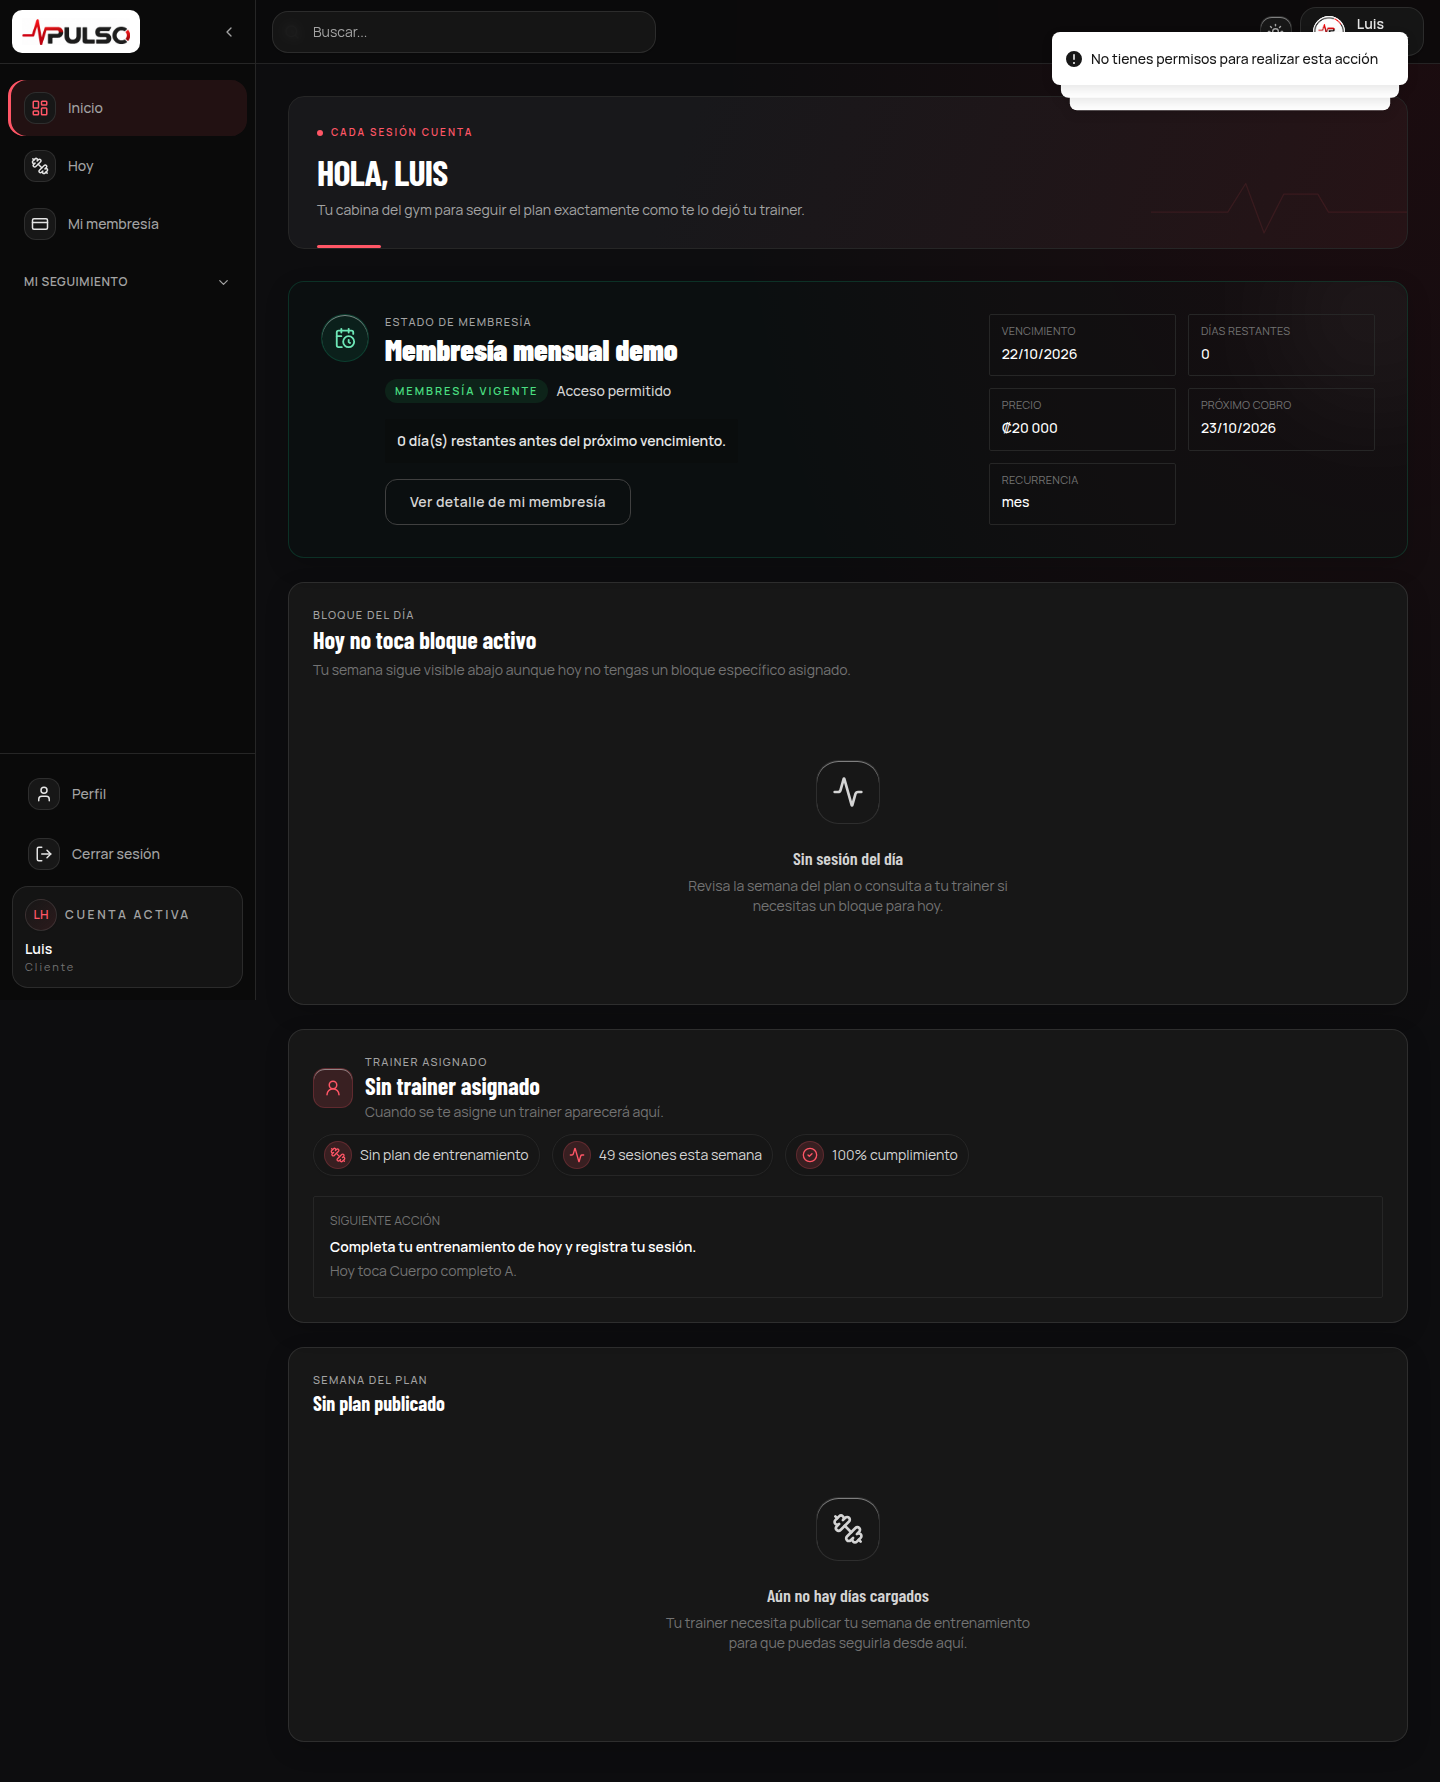
\includegraphics[width=0.92\textwidth]{imagenes/captura_actual_panel_cliente.png}
\caption{Panel de seguimiento del cliente}
\caption*{\textit{Nota}. Captura propia de la versión local de demostración con datos ficticios, 23 de septiembre de 2026.}
\end{figure}

\Needspace{8\baselineskip}
\subsection{Procedimiento para capturas responsive}

El repositorio incorpora \texttt{frontend/capturar\_anexos.mjs}, que usa
Playwright y Chromium para capturar las funciones de administración, instructor
y cliente en escritorio, además de vistas móviles. Esta actualización incorpora
una vista representativa de cada interfaz. La ejecución usa cuentas y datos
ficticios; no emplea datos de gimnasios ni modifica el despliegue público.

\subsection{Trazabilidad del análisis financiero}\label{ap:presupuesto}

Los cálculos del informe son de elaboración propia a partir del escenario
financiero preliminar. El equipo usó una hoja de cálculo como borrador de
trabajo; las tablas incluidas aquí presentan los montos y supuestos necesarios
para revisar la proyección. Antes de ofrecer el servicio se comprobarán los
precios con cotizaciones y se completarán los costos de impuestos, comisiones,
formalización y consumo adicional de nube. Las tarifas oficiales y sus
condiciones se reúnen en la Sección~\ref{sec:fuentes-precios}; cada proveedor
aparece citado en la bibliografía.

\begin{table}[htbp]
\caption{Supuestos principales del análisis financiero de Pulso}
\begin{tabularx}{\textwidth}{>{\bfseries}p{4.3cm}r X}
\toprule
Concepto & Importe o nivel & Supuesto \\
\midrule
Gastos fijos y trabajo valorado & 114\,247,54 & Base mensual del escenario preliminar. \\
Costo de desarrollo & 198\,735,27 & Trabajo propio valorado; no desembolso inicial. \\
Liquidez inicial mínima & 40\,000 & Reserva de efectivo proyectada. \\
Soporte y nube & Variable & Se ajusta por cartera, altas y consumo proyectado. \\
\midrule
Punto de equilibrio operativo & 6 clientes & Primer resultado mensual positivo en el escenario. \\
\bottomrule
\end{tabularx}
\caption*{\textit{Nota}. Elaboración propia a partir del escenario financiero preliminar. Montos por confirmar antes de la venta.}
\end{table}

\subsection{Referencias de despliegue demostrativo}

\begin{itemize}
  \item Frontend: \url{https://proyectoappgym-frontend.vercel.app}
  \item Backend: \url{https://proyectoappgym-backend.vercel.app}
  \item Documentación API: \url{https://proyectoappgym-backend.vercel.app/api/docs/}
\end{itemize}

No se incluyen credenciales en el documento público. Durante la demostración se
utilizarán cuentas preparadas por el equipo y datos ficticios.
